\documentclass[12pt]{article}
\usepackage{graphicx}
%\documentclass[journal,12pt,twocolumn]{IEEEtran}
\usepackage[none]{hyphenat}
\usepackage{graphicx}
\usepackage{listings}
\usepackage[english]{babel}
\usepackage{graphicx}
\usepackage{caption}
\usepackage{hyperref}
\usepackage{booktabs}
\usepackage{array}
\usepackage{amsmath}   % for having text in math mode
\usepackage{listings}
\lstset{
  frame=single,
  breaklines=true
}
%New macro definitions
\newcommand{\mydet}[1]{\ensuremath{\begin{vmatrix}#1\end{vmatrix}}}
\providecommand{\brak}[1]{\ensuremath{\left(#1\right)}}
\providecommand{\norm}[1]{\left\lVert#1\right\rVert}
\newcommand{\solution}{\noindent \textbf{Solution: }}
\newcommand{\myvec}[1]{\ensuremath{\begin{pmatrix}#1\end{pmatrix}}}
\let\vec\mathbf

\begin{document}
\begin{center}
\textbf\large{CLASS-10\\CHAPTER-7 \\ COORDINATE GEOMETRY}
\end{center}

\section*{EXERCISE - 7.1}
\begin{enumerate}
	\item The distance of the point $\vec{P}(2, 3)$ from the x-axis is

\begin{enumerate}
\item 2
\item 3
\item 1
\item 5 
\end{enumerate}
\item The distance between the points $\vec{A}(0, 6) \text{ and } \vec{B}(0, –2)$ is
	\begin{enumerate}
\item 6
\item 8
\item 4	
\item 2
	\end{enumerate}
\item The distance of the point $\vec{P} (–6, 8)$ from the origin is
\begin{enumerate}

\item 8
\item 2$\sqrt{7}$ 
\item 10
\item 6
\end{enumerate}
\item The distance between the points $\vec(0, 5)\text{ and }(–5, 0)$ is
\begin{enumerate}

\item 5
\item 5
\item 5
\item 10
\end{enumerate}
\item $\vec{AOBC}$ is a rectangle whose three vertices are vertices $\vec{A} (0, 3), \vec{O}(0, 0)\text{ and }
	\vec{B} (5, 0)$. The length of its diagonal is
\begin{enumerate}
\item 5
\item3
\item 34
\item 4
\end{enumerate}
\item The perimeter of a triangle with vertices $\vec(0, 4), (0, 0) \text{ and } (3, 0)$ is
\begin{enumerate}

\item5
\item 12
\item 11
\item 7
\end{enumerate}
\item The area of a triangle with vertices $\vec{A}(3, 0), \vec{B}(7, 0) \text{ and } \vec{C}(8, 4)$ is
\begin{enumerate}

\item 14
\item 28
\item 8
\item 6
\end{enumerate}
\item The points $ (–4, 0), (4, 0), (0, 3) $are the vertices of
	\begin{enumerate}
\item right triangle 
\item isosceles triangle
\item  equilateral triangle
\item  scalent triangle 
\end{enumerate}
\item The point which divides the line segment joining the points $\vec{P} (7, –6) \text{ and } (3, 4)$ in
ratio 1 : 2 internally lies in the
\begin{enumerate}

\item I quadrant

\item  II quadrant

\item  III quadrant

\item  IV quadrant
\end{enumerate}

\item The point which lies on the perpendicular bisector of the line segment joining the
	points $\vec{A} (–2, –5)\text { and } \vec{B} (2, 5) $is
\begin{enumerate}
\item  	$(0, 0)$
\item  $(0, 2)$ 
\item  $(2, 0)$ 
\item  $(–2, 0)$
\end{enumerate}
\item The fourth vertex $\vec{D}$ of a parallelogram $\vec{ABCD}$ whose three vertices are
	$\vec{A} (–2, 3), \vec{B} (6, 7)\text { and } \vec{C} (8, 3)$ is
\begin{enumerate}
	\item $(0, 1)$
	\item $(0, –1)$
	\item $ (–1,0)$
	\item$(1, 0)$
\end{enumerate}
\item If the point $\vec{P} (2, 1)$ lies on the line segment joining points$\vec{A} (4, 2) \text{ and } \vec{B} (8, 4)$,
then
\begin{enumerate}
	\item $\vec{AP} =\frac{1}{3}\vec{AB}$ 
\item $\vec{AP}=\vec{PE}$
\item $\vec{PB}=\frac{1}{3}\vec{AB}$
\item$\vec{AP}=\frac{1}{2}\vec{AB}$
 \end{enumerate}
 \item If P $\frac{a}{3}$ is the mid-point of the line segment joining the points $\vec{Q} (– 6, 5) \text{ and }(– 2, 3),$ then the value of a is
\begin{enumerate}
\item – 4
\item – 12
\item 12
\item – 6
\end{enumerate}

\item The perpendicular bisector of the line segment joining the points $\vec{A} (1, 5) \text{ and }
\vec{B} (4, 6)$ cuts the y-axis at
\begin{enumerate}
	\item$(0, 13)$ 
	\item $(0, –13)$
	\item$(0, 12) $
	\item$(13, 0)$
\end{enumerate}
\item The coordinates of the point which
	is equidistant from the three vertices of the  $\vec{AOB}$ as shown in the
vFig. 7.1 is
\begin{enumerate}
	\item $(x, y)$
	\item $(y, x)$
	\item $(\frac{x}{2},\frac{y}{2})$
\item $(\frac{y}{2},\frac{x}{2})$
\end{enumerate}
\item A circle drawn with origin as the
centre passes through 
$(\frac{13}{2},0)$. The
point which does not lie in the
interior of the circle is
\begin{enumerate}
\item $(\frac{-3}{4},1)$
\item $(2,\frac{7}{3})$
\item $(5,\frac{-1}{2})$
\item $(-6,\frac{-5}{2})$
\end{enumerate}
\item A line interects the y-axis and x-axis of the points $\vec{P} \text{ and }\vec{Q}$, respectiveiy.lf $(2,5)$is the mid-point of $\vec{PQ}$.then the coordinates of $\vec{P} \text{ and } \vec{Q}$ are,respectively
\begin{enumerate}
	\item$(0,-5)\text{ and }(2,0)$
	\item$(0,-10)\text{ and }(-4,0)$
	\item$(0,4)\text{ and } (-10,0)$
	\item$(0,-10)\text{ and }(4,0)$
\end{enumerate}
\item The area of a triangle with vertices $(a,b+c), (b,c+a)\text{ and }(c,a+b)$ is
\begin{enumerate}
\item $(a+b+c)^2$
\item 0
\item a+b+c
\item abc 
\end{enumerate}
\item If the distance between the points $(4,P) \text{ and } (1,0)$ is 5,then the value of $\vec{P}$ is
\begin{enumerate}                       
\item4 only
\item+4 only
\item-4 only
\item0
\end{enumerate}
\item lf the points $\vec{A}(1,2),\vec{0}(0,0)\text{ and }\vec{C}(a,b)$ are collinear,then
\begin{enumerate}
\item a=b
\item a=2b
\item 2a=b
\item a=-b
\end{enumerate}
\begin{figure}[h!]
  \centering
  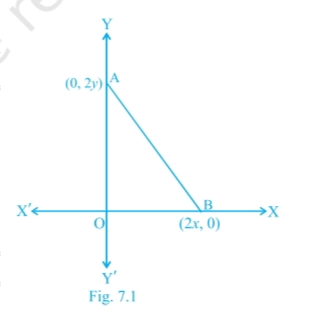
\includegraphics[width=\columnwidth]{./figs/image.jpg}
  \caption{}
\label{fig:10/7/12Fig1}
\end{figure}

	\end{enumerate}
	\end{document}


 

 





 

 

